\documentclass[8pt]{standalone}
\usepackage{pgfplots}
\pgfplotsset{compat=1.18}


\begin{document}
	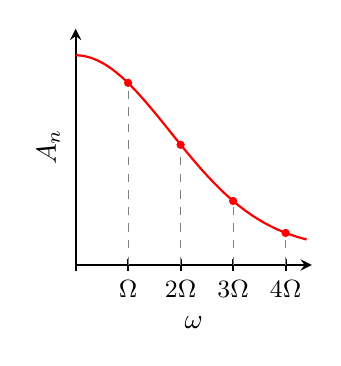
\begin{tikzpicture}
		\begin{axis}[
			width=3cm,
			height=3cm,
			xlabel={$\omega$},
			ylabel={$A_n$},
			ytick=\empty,
			xmin=0, xmax=4.5,
			ymin=0, ymax=4.5,
			axis lines=left,
			axis line style={-stealth, thick, black},
			tick style={black, thick},
			xtick={0, 1, 2, 3, 4, 5},
			xticklabels={$ $, {\small $\Omega$}, {\small $2\Omega$}, {\small $3\Omega$}, {\small $4\Omega$}, {\small $5\Omega$}},
			scale only axis
			],
			
			\addplot[domain=0:4.4, samples=100, thick, red]{
				0.3 + 1/(0.108*sqrt(2 * pi)) * exp(-(x^2)/(60*0.108))
			};
			
			\draw[dashed, gray] (1,0) -- (1,3.47);  
			\draw[dashed, gray] (2,0) -- (2,2.29);  
			\draw[dashed, gray] (3,0) -- (3,1.22);  
			\draw[dashed, gray] (4,0) -- (4,0.61);  
			
			\fill[red] (1,3.47) circle (1.5pt);
			\fill[red] (2,2.29) circle (1.5pt);
			\fill[red] (3,1.22) circle (1.5pt);
			\fill[red] (4,0.61) circle (1.5pt);
		\end{axis}
	\end{tikzpicture}
\end{document}